
\subsection{Performance de MPTCP sur mininet}
\label{sec:CR:perfMPTCP:base}

Apr�s la compilation du noyau, pour v�rifier le fonctionnement de
MPTCP nous avons mesurer le d�bit moyen en utilisant \emph{iperf} sur
la topologie A.

Les param�tres du r�seau sont les suivants.

\vspace{1cm}
\begin{tabular}{lp{\linewidth - 4cm}}

\textbf{fichier}& \textbf{Commentaires}\\
\hline
MSS& 1460 Bytes\\
Window size& \\
d�lai par lien & 10 ms\\
\end{tabular}
\vspace{0.5cm}






Les performances de TCP ou de MPTCP d�pendent des param�tres utilis�s
dans la connexion entre deux h�tes. En particulier, le d�bit de chaque
chemin, le d�lai (RTT) sont des facteurs un r�le important dans le d�bit moyen
mesur�. Afin de d�terminer les limites de notre simulation, nous avons
utilis� la topologie simple pour caract�riser les performances de
MPTCP sur plusieurs sous-flots o� chacun des liens de la topologie
poss�de les m�mes propri�t�s (d�bit maximal, RTT, perte, gigue).

Pour mesurer la performance maximale obtenue avec cette topologie,
nous utilisons l'application iperf.

\begin{figure}[!htb]
  \begin{changemargin}{-2.0cm}{0.5cm}
    \centering
    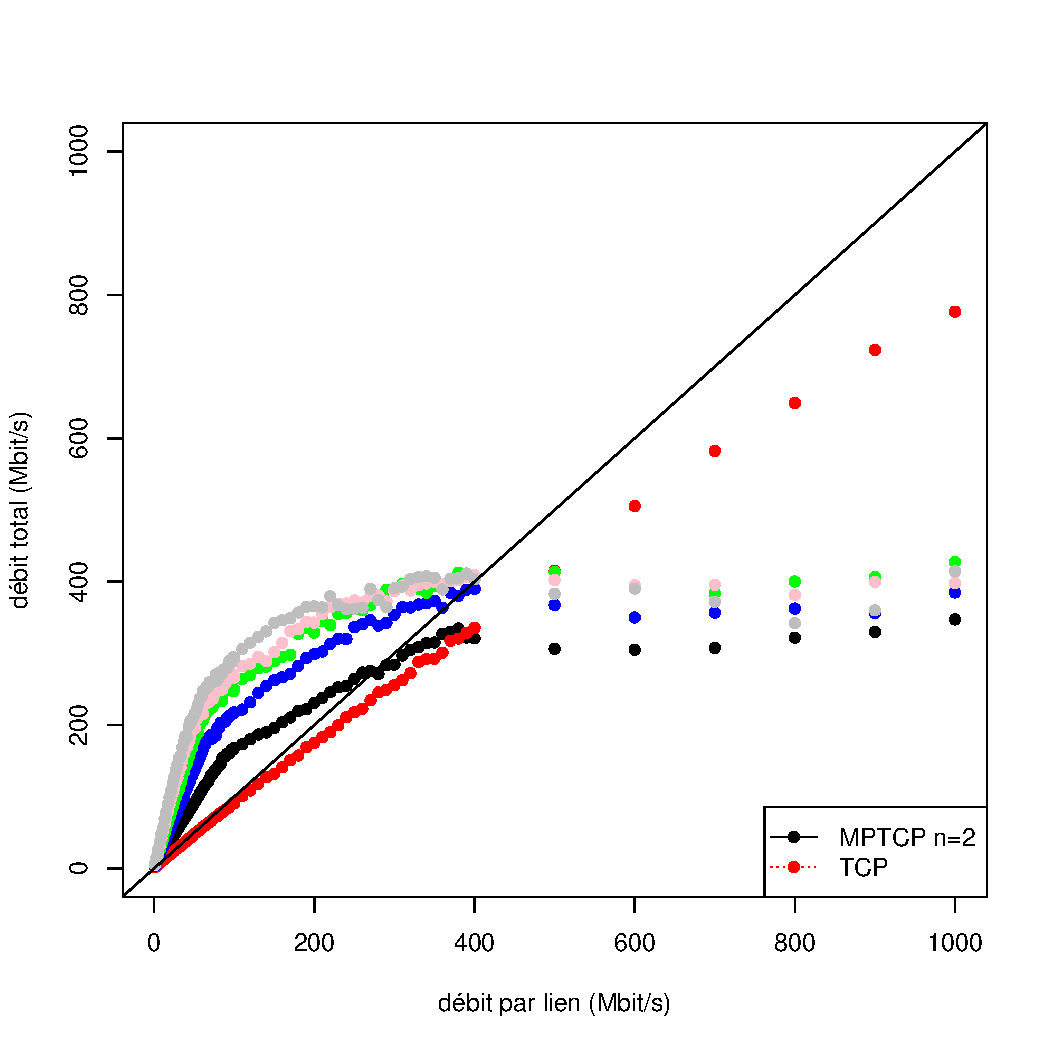
\includegraphics[width=0.7\textwidth]{../figures/bw.pdf}
  \end{changemargin}
  \centering
  
  \caption{\textbf{Sch�ma de la pile MPTCP}. source : \url{www.cisco.org}}
  \label{fig:mptcpstack}
  
\end{figure}